% Writing template based on OpacityCalculation_v2_structure.tex.
% Italic outline notes are writing instructions, not manuscript prose.
% Existing figures and equations are retained; v2 is unchanged.
\documentclass[final,5p,times,twocolumn]{elsarticle}

\usepackage{amssymb}
\usepackage{amsmath}
\usepackage{graphicx}
\usepackage{url}
\usepackage[colorlinks=true, urlcolor=blue, linkcolor=blue, citecolor=blue]{hyperref}

\makeatletter
\setlength{\@fptop}{0pt}
\setlength{\@fpbot}{0pt plus 1fil}
\makeatother

\DeclareRobustCommand{\secref}[1]{\hyperref[#1]{Section~\ref*{#1}}}
\DeclareRobustCommand{\figref}[1]{\hyperref[#1]{Figure~\ref*{#1}}}
\DeclareRobustCommand{\eqnref}[1]{\hyperref[#1]{Eq.~(\ref*{#1})}}
\newcommand{\draft}[1]{\par\noindent\textit{Outline: #1}\par\medskip}

\renewcommand{\ttdefault}{lmtt}
\journal{High Energy Density Physics}

\begin{document}
\begin{frontmatter}

\author[1]{Roy G. Yaron}
\cortext[cor1]{Corresponding author: \href{mailto:udini@tauex.tau.ac.il}{udini@tauex.tau.ac.il}}
\affiliation[1]{organization={School of Physics and Astronomy, Tel Aviv University},
           city={Tel Aviv}, postcode={6997801}, country={Israel}}

\title{Expansion-Aware Gray Opacities for Supernova and Kilonova Radiation Transport}

\begin{abstract}
    In expanding ejecta photons shift through spectral lines, making it difficult to describe radiation transport 
    with a single Rosseland opacity, as needed for analytical models and simplified simulations.
    We show that the Rosseland mean of a mean free path based expansion opacity provides
    a good approximation to radiation transport in expanding ejecta. Combining a finite-bin
    implementation of the Karp et al. transport prescription with an absorption Planck mean
    derived from saturated frequency-bin-averaged opacity, single-group Monte Carlo calculations
    reproduce multigroup luminosity curves, with peak luminosities differing by $7$--$33\%$.
    This agreement supports a physically motivated gray description while reducing simulation
    time by approximately two orders of magnitude for lanthanide-rich models. We use this
    framework to investigate the temperature, density, and composition dependence of the
    transport opacity in kilonova ejecta and identify a representative value above the diffusion
    surface. For an eight-element mixture based on solar $r$-process abundances, averaging over
    the cooling interval $0.2<T_{\rm diff}<1$~eV gives
    $\kappa_{\rm avg}\simeq(0.197+93.82X_{\rm lan}^{0.691})$~cm$^2$~g$^{-1}$,
    where $X_{\rm lan}$ is the lanthanide mass fraction. This relation connects ejecta composition
    to the effective opacity governing the modeled kilonova emission.
    \end{abstract}

\begin{keyword}
    expansion opacity \sep Rosseland mean \sep kilonova \sep Type Ia supernovae
\end{keyword}

\end{frontmatter}


\section{Introduction}
\label{SecIntro}

    In expanding plasmas, due to the Doppler effect, as photons travel through the plasma, their frequency changes. 
    This effect is mainly important for bound-bound transitions, because their narrow line structure in frequency causes photons to interact 
    with different lines as they travel through the plasma.
    This effect is known as expansion opacity, and it is important for many astrophysical applications, such as Type Ia supernovae,
    kilonovae and stellar winds. 

    For non-moving plasmas, the radiation flux can be approximated well using the Rosseland mean opacity, which is a weighted
    average of the opacity over all frequencies. However, for expanding plasmas with significant bound-bound opacity, the Rosseland mean 
    opacity is not a good approximation, since the width of the bound-bound lines is negligible and photons interact with them only due to their
    frequency change as they travel through the plasma. 
    Therefore the average distance a photon travels cannot be derived from $\kappa(\nu)$
    alone because it inherently depends on the photon's direction of movement and the plasma's velocity gradient.
    To avoid this problem and to allow calculation of transport that can inherently depend on the photon's direction of movement and
    velocity gradient, radiation transport in systems with expansion opacity is usually calculated using Monte Carlo simulations,
    which track individual photons and their frequency evolution as they propagate through the expanding medium.

    Calculating an effective Rosseland mean opacity has several motivations: a single opacity value 
    (1) is required for analytic 
    models and closed-form solutions, which cannot treat full frequency-dependent opacity; (2) gives direct physical 
    intuition for how temperature and composition affect the opacity and hence the light curve; and (3) enables 
    faster and simpler simulations than full frequency-dependent calculations. 

    Previous attempts to address this problem have been proposed. Fontes et al. \cite{fontes2015opacity,fontes2017linesmeared}
    suggested using artificial 
    line broadening by assigning a line width corresponding to unphysical high temperature of 20 MeV, 
    which effectively smears the bound-bound lines 
    over a finite frequency range. This approach preserves the integral of the opacity over
    frequency (area-preserving line profiles) and for kilonova ejecta it  
    produces frequency-dependent opacities that are one to two orders of magnitude greater than those
    obtained with expansion opacities in 
    the Sobolev approximation without broadening. Fontes et al. \cite{fontes2020opacity} demonstrated that
    their smeared opacity tables, 
    calculated using the Sobolev formalism, yield light curves for multigroup radiative transfer simulations
    that are similar to those 
    obtained from full line-by-line Monte Carlo radiation transport (using the superNu code) for kilonovae.
    However, this approach still requires multigroup frequency-dependent opacity tables rather than
    a single gray (frequency-averaged) Rosseland mean opacity and uses an unphysical assumption that
    has been verified only for specific ejecta.
    Several works \cite{deprince2024kilonova,just2022properties,tanaka2020systematic} have shown how opacity depends on composition,
    temperature, density, and time by comparing the Planck mean expansion opacity over those parameters.
    The Planck mean is nevertheless not the appropriate average for the opacity that controls photon
    escape from the ejecta. In a non-expanding medium this transport opacity is the Rosseland mean,
    which weights the low-opacity frequency windows through which photons preferentially diffuse.
    In an expanding medium the same transport character is needed, but the opacity must also include
    the line absorption encountered as the photon redshifts through the expanding flow.

    In this paper we present the effective expansion opacity, $\kappa_{\rm exp}$, which accounts for
    bound-bound expansion opacity. The method follows an outward-moving photon in homologous expansion
    ($r=vt$) and calculates the distance over which it reaches optical depth $\tau\simeq1$.
    Taking the Rosseland mean of $\kappa_{\rm exp}$ defines the effective expansion Rosseland mean,
    $\kappa_R^{\rm exp}(T,\rho,t)$.
    This gray-opacity method assumes that the photons dominating the diffusion are close to a
    blackbody spectrum. It is therefore useful for bolometric luminosities and characteristic
    temperatures, but not for detailed line spectra.

\section{Expansion Opacity Formalisms}
\label{SecExpansion}

\subsection{Mean Free Path Based Expansion Opacity}
\label{SecMeanFreePath}
\draft{Present Karp's construction: photon redshift through successive lines, cumulative attenuation by lines and continuum, and the resulting effective mean free path and opacity. Give the assumptions and Rosseland-mean definition. Keep finite-bin modifications for Section~\ref{SecFrequencyConvergence}.}

\subsection{Frequency-Bin-Averaged Expansion Opacity}
\label{SecBinAveraged}
\draft{Present the frequency-bin sum of Sobolev interaction probabilities, $1-e^{-\tau_l}$, and its physical interpretation. Cite the stellar-wind antecedents and Eastman--Pinto application. Explain the distinction from the mean-free-path construction; define the Planck mean without claiming that this prescription is universally accurate for emission.}
\draft{Use Figure~\ref{fig:BB_line_example} to illustrate the spectral differences. Check that the plotted curves and legend match the definitions; any finite-bin hybrid belongs to Section~\ref{SecFrequencyConvergence}.}

\begin{figure}[t]
    \centering
    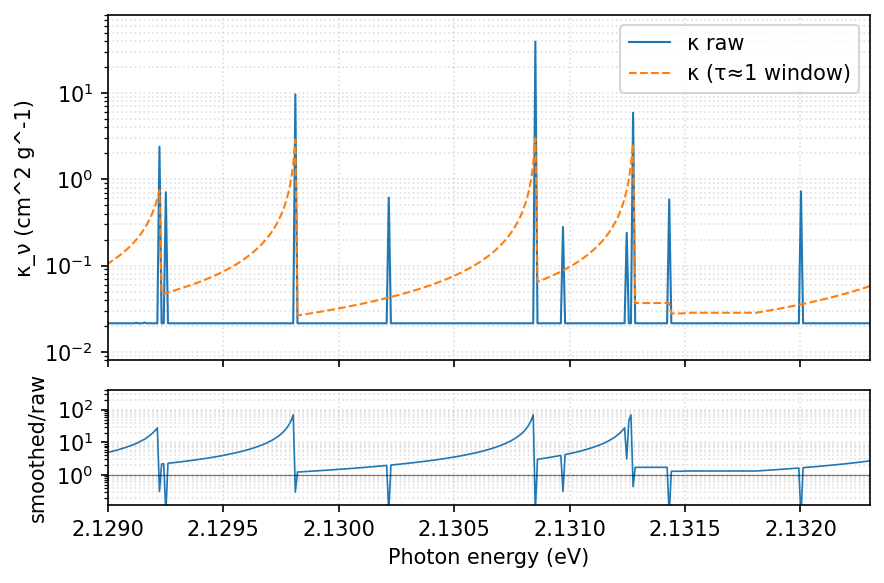
\includegraphics[width=\columnwidth]{figs/kappa_smoothed_vs_raw_error.png}
    \caption{Spectral opacity comparison at a single thermodynamic point for Fe.}
    \label{fig:BB_line_example}
\end{figure}

\clearpage
\section{Numerical Accuracy of Rosseland-Mean Transport}
\label{SecRadiationSimulations}

\subsection{Frequency Discretization and Convergence}
\label{SecFrequencyConvergence}
\draft{Describe the finite-frequency-bin implementation, redward propagation, and continuum treatment. Specify the optical-depth criterion and saturated-opacity replacement for a single optically thick bin. Identify this as the numerical prescription used here, not an unchanged implementation of Karp's formalism.}
\draft{Compare the Rosseland means as frequency resolution changes for Fe and Er in Figure~\ref{fig:convergence}. Report the tested conditions, convergence, and coarse-bin differences quantitatively. Do not infer random line positions or general accuracy from agreement in these two tests alone.}

\begin{figure}[t]
    \centering
    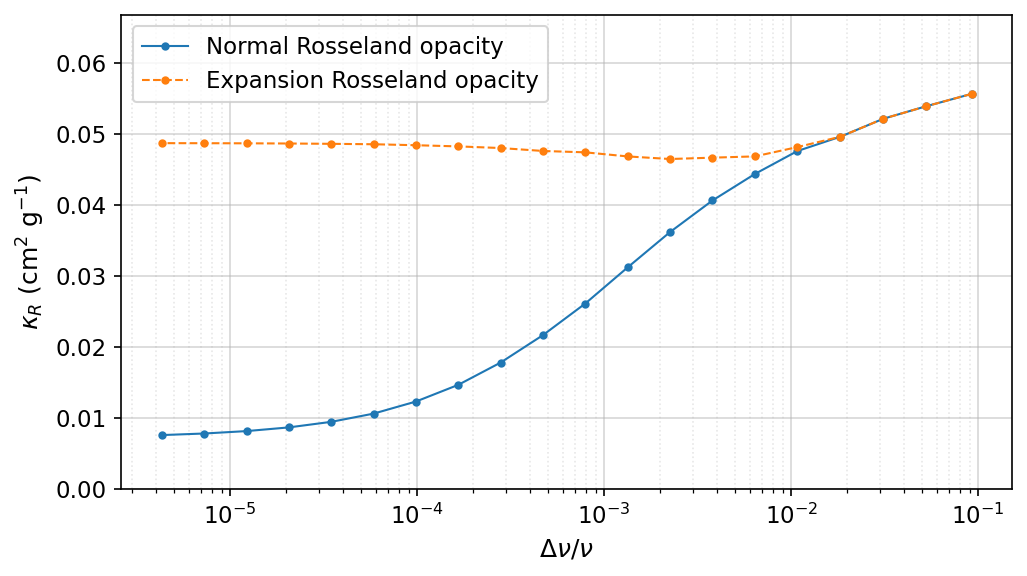
\includegraphics[width=\columnwidth]{figs/convergence_Fe_rho1.00e-12_t3.0days.png}\\[0.5em]
    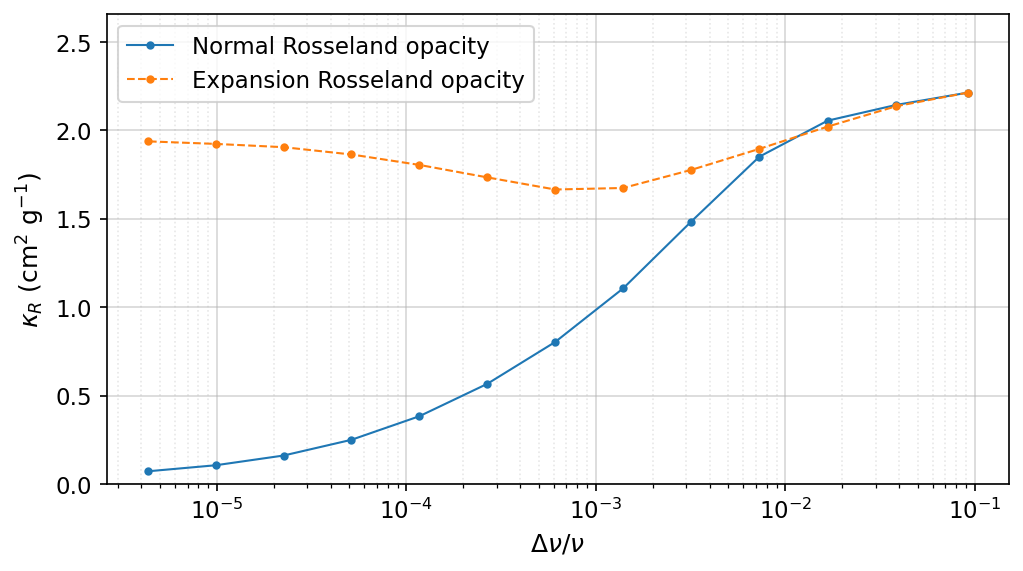
\includegraphics[width=\columnwidth]{figs/convergence_Er_rho1.00e-12_t1.0days.png}
    \caption{Dependence of the Rosseland mean opacity on frequency-bin width
    for Fe (top) and Er (bottom), comparing the frequency-bin-averaged
    prescription with the binned mean-free-path-based implementation.}
    \label{fig:convergence}
\end{figure}

\clearpage
\subsection{Single-Group versus Multigroup Monte Carlo Transport}
\label{SecTransportSetup}
\label{SecTemperatureStructure}
\draft{Describe the common URILIGHT setup: ejecta profiles, compositions, heating and deposition, initial conditions, and temperature calculation. Specify the opacity tables and absorption/scattering treatment. Explain the use of the mean-free-path-based Rosseland mean for transport and the frequency-bin-averaged absorption Planck mean for thermal coupling as a modeling choice to be tested.}
\draft{Compare luminosity curves in Figure~\ref{fig:comparison}. Define the escaping-radiation temperature estimator and the single-group temperature proxy before comparing them in Figure~\ref{fig:trad_vs_phot}. Distinguish differences in the estimators from differences between transport methods.}
\draft{Define the diffusion and thermalization/photospheric surfaces used to interpret the temperature comparison and the later applications. State the optical-depth and diffusion-time criteria explicitly. Summarize agreement, limitations, and measured computational cost, including table construction.}

\begin{figure*}[t]
    \centering
    \includegraphics[width=\textwidth]{figs/luminosity_models.png}
    \caption{Single-group versus multigroup bolometric luminosity for
    Type Ia supernova and kilonova models with different $X_{\rm lan}$.}
    \label{fig:comparison}
\end{figure*}

\begin{figure}[t]
    \centering
    \includegraphics[width=\columnwidth]{figs/trad_vs_phot.png}
    \caption{Escape-averaged $T_{\rm rad}$ (multigroup) versus plasma $T$ at
    $\tau_{\rm abs}(1+\tau_{\rm scat})=1$ (single-group).}
    \label{fig:trad_vs_phot}
\end{figure}

\clearpage
\section{Rosseland-Mean Opacities of r-Process Ejecta}
\label{SecTypicalOpacity}

\subsection{Composition and Thermodynamic Dependence}
\label{SecCompositionTrends}
\draft{Introduce the atomic databases and the eight-element mixture based on solar $r$-process abundances. Describe the abundance source, conversion from number abundance to mass, restriction to $90<A\leq215$, and mapping of eight mass-number windows onto Zr, Ru, Xe, Nd, Eu, Er, Re, and Pb using Figure~\ref{fig:kilonova_composition}. Define $X_{\rm lan}$, normalization, and rescaling of the lanthanide and non-lanthanide components at fixed relative proportions within each group; state the omission of actinides.}
\draft{Discuss the temperature, density, time, and composition dependence of the Rosseland mean. Use Figure~\ref{fig:kappa_composition_slices} for the density dependence and the opacity minimum near $1$--$1.5$~eV. Defer the time-dependent and observable implications to Section~\ref{SecEarlyFeature}.}

\begin{figure}[t]
    \centering
    \includegraphics[width=\columnwidth]{figs/kilonova_composition.png}
    \caption{Cumulative mass of the solar $r$-process abundance pattern over
    $90<A\leq215$, with the eight representative elements and their mass fractions.}
    \label{fig:kilonova_composition}
\end{figure}

\begin{figure*}[t]
    \centering
    \includegraphics[width=\textwidth,height=0.36\textheight,keepaspectratio]{figs/kappa_composition_slices.png}
    \caption{Mixture $\kappa_R^{\rm exp}(T)$ and $\kappa_R^{\rm exp}(\rho)$
    slices for different kilonova compositions, with a Type Ia composition
    included for comparison.}
    \label{fig:kappa_composition_slices}
\end{figure*}

\clearpage
\subsection{Time Evolution and Representative Ejecta Opacities}
\label{SecOpacityEvolution}
\draft{Use the surfaces defined in Section~\ref{SecTransportSetup} to interpret the temperature and opacity maps for $X_{\rm lan}=0.1$ in Figure~\ref{fig:profile_colormap}. Show the diffusion-surface velocity, temperature, and density in Figure~\ref{fig:kilonova_diffusion_surface}. Discuss changes associated with the adopted density profile.}
\draft{Define the column-density-weighted opacity above the diffusion surface using Eq.~\ref{eq:kappa_avg}, and show its time evolution in Figure~\ref{fig:diffusion_opacity_evolution}. Distinguish the local Type Ia opacity in that figure from the averaged kilonova opacity.}

\begin{equation}
    \label{eq:kappa_avg}
    \kappa_{\rm avg}(t)
    =
    \frac{\displaystyle\int_{v_{\rm diff}}^{v_{\rm max}}
        \kappa_R^{\rm exp}\,\rho\,t\,dv}
         {\displaystyle\int_{v_{\rm diff}}^{v_{\rm max}}\rho\,t\,dv}
    =
    \frac{\tau(v_{\rm diff})}{\Sigma(v_{\rm diff})}.
\end{equation}

\draft{Define the average over the cooling interval $0.2<T_{\rm diff}<1$~eV with weights in $\ln t$, only where the diffusion surface is defined. Present the composition fit and its sensitivity to ejecta profiles in Figure~\ref{fig:kappa_xlan}. Check the retained fit coefficients against the current data before finalizing.}

\begin{equation}
    \label{eq:kappa_xlan}
    \kappa_{\rm avg}(X_{\rm lan})
    = \left(0.197 + 93.82\,X_{\rm lan}^{0.691}\right)
    \ {\rm cm^{2}\,g^{-1}}.
\end{equation}

\begin{figure*}[t]
    \centering
    \includegraphics[width=\textwidth]{figs/kilonova_lan10_profile_colormap.png}
    \caption{Kilonova plasma-temperature and Rosseland-opacity maps for
    $X_{\rm lan}=0.1$, with diffusion and photospheric surfaces overlaid.}
    \label{fig:profile_colormap}
\end{figure*}

\begin{figure*}[t]
    \centering
    \includegraphics[width=\textwidth,height=0.72\textheight,keepaspectratio]{figs/kilonova_diffusion_surface.png}
    \caption{Diffusion-surface velocity, temperature, and density versus time
    for six kilonova lanthanide mass fractions $X_{\rm lan}$.}
    \label{fig:kilonova_diffusion_surface}
\end{figure*}

\begin{figure*}[t]
    \centering
    \includegraphics[width=\textwidth]{figs/kilonova_diffusion_surface_opacity.png}
    \caption{Opacity versus time: local Rosseland opacity at the Type Ia
    diffusion surface (left) and column-density-weighted opacity above the
    kilonova diffusion surface (right). Black markers delimit the sampled
    cooling interval $0.2<T_{\rm diff}<1$~eV, truncated where the diffusion
    surface becomes undefined.}
    \label{fig:diffusion_opacity_evolution}
\end{figure*}

\begin{figure*}[t]
    \centering
    \includegraphics[width=\textwidth,height=0.36\textheight,keepaspectratio]{figs/kappa_vs_xlan.png}
    \caption{$\kappa_{\rm avg}$ versus $X_{\rm lan}$ for five ejecta profiles and
    a global fit, averaging in $\ln t$ over $0.2<T_{\rm diff}<1$~eV where the
    diffusion surface is defined. Error bars show the weighted temporal
    standard deviation.}
    \label{fig:kappa_xlan}
\end{figure*}

\clearpage
\subsection{A Possible Early-Time Signature of the Opacity Increase}
\label{SecEarlyFeature}
\draft{Connect the time-dependent opacity increase during cooling below about $1$~eV to the early luminosity decline in the high-lanthanide models. Use Figures~\ref{fig:diffusion_opacity_evolution} and \ref{fig:comparison}; distinguish a correlation from a demonstrated causal or observable signature.}
\draft{Use Figure~\ref{fig:all_lanthanides_opacity} to test sensitivity to element choice and atomic data. Describe the general HRF Rosseland-opacity decrease from roughly $1$ to $1.5$~eV, including exceptions and its weaker presence in the Planck mean. Explain that the black curves represent an equal-atomic-fraction mixture, not an arithmetic average of individual opacities. State that the Ho/Er/Tm HULLAC comparison only partially recovers the trend, so database independence is not established.}
\draft{Possible additional work: compare with a constant-opacity, power-law-density light-curve model and test whether the evolving opacity can constrain the lanthanide fraction. Keep this interpretation provisional until tested.}

\begin{figure*}[t]
    \centering
    \includegraphics[width=\textwidth]{figs/lanthanide_opacity_main.png}
    \caption{Temperature dependence of (a) Rosseland and (b) total Planck mean
    opacities for individual lanthanides in the HRF database. Black curves show
    a mixture of all lanthanides with equal atomic number fractions.
    (c) Rosseland opacities for Ho, Er, and Tm from HRF and HULLAC.}
    \label{fig:all_lanthanides_opacity}
\end{figure*}

\clearpage
\end{document}
